\chapter{Method}
\label[chapter]{chapter:method}

This chapter outlines the method of the pipeline developed during this project in order to solve the task at hand. Details regarding the general logic of each component are described in detail, while practical implementation details will be covered in the next chapter.

To simplify, the method can be divided into four main components: railway processing, track detection, track reprojection, and error minimization. \Cref{fig:method_overview} shows an overview of these main components, the overall inputs/outputs to the pipeline (classified by type), and the interactions between the components. Each component box also specifies how often that component is executed and what the component goal/output are.

\begin{figure}[h]
\begin{center}
    \label[figure]{fig:method_overview}
    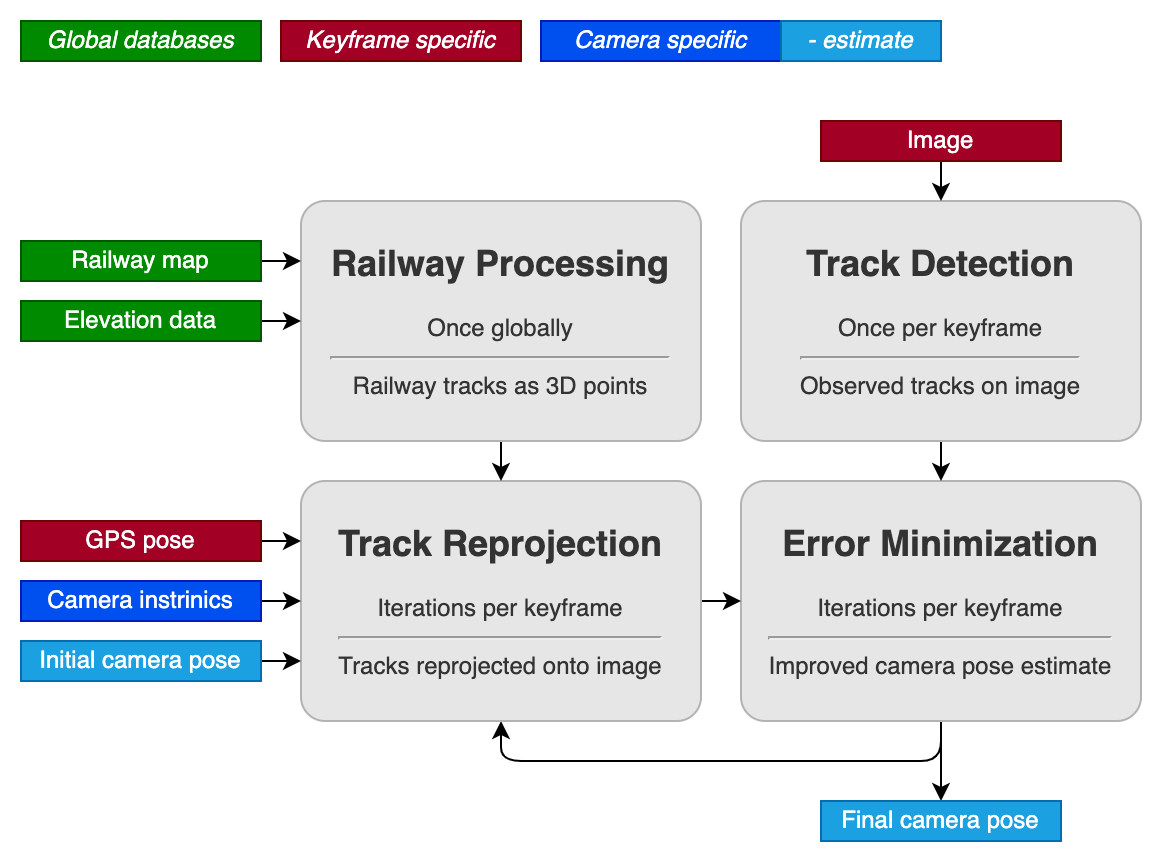
\includegraphics[width=\textwidth]{images/overview}
    \caption{Overview of main components, their interactions, and inputs/outputs.}
\end{center}
\end{figure}


\section{Railway Processing}
\label[section]{sec:railway_processing}

In this component, a railway map (data from an OSM file) is processed in order to obtain a set of relevant global 3D points that represent the railway tracks. This is done by extracting the nodes and tracks from the railway map, converting the nodes to points sorted by tracks, then filling the gaps between the points to achieve more regular spacing, and adding elevation data to get 3D points.

\begin{multicols}{2}
    \textbf{Inputs}
    \begin{itemize}
        \item Railway map (OSM data)
        \item Elevation data
    \end{itemize}
    
    \textbf{Outputs}
    \begin{itemize}
      \item Railway: tracks as 3D points
    \end{itemize}

    \vfill\null
    \columnbreak

    \textbf{Process}
    \begin{enumerate}
        \item Extract nodes and tracks from railway map
        \item Convert nodes to points per track
        \item Fill track gaps by 2D interpolation
        \item Add elevation data to get 3D points
    \end{enumerate}
\end{multicols}

Overall, the initial data is enhanced, while also being reduced to what is actually needed for downstream components -- only in the relevant area that is a combined map of all specified keyframes. Even though processing a combined map of all keyframes takes more time once, it is much faster than processing the railway surrounding each keyframe location individually, since points may overlap. Moreover, this is the only way to ensure that large railway gaps do not lead to a problem of missing data in the view of any single keyframe.

\section{Track Reprojection}
\label{sec:track_reprojection}

In this component, the railway points ahead of the current keyframe GPS location are reprojected into the image. This is done by first selecting railway tracks with local points from the global railway tracks, transforming these points into the camera frame, then filtering the points by distance from the camera (to obtain a more regular spacing in image space), and finally reprojecting these points into the image space.

\begin{multicols}{2}
    \textbf{Inputs}
    \begin{itemize}
        \item Railway: tracks as 3D points
        \item Keyframe: GPS pose
        \item Camera: intrinsics
        \item Camera: pose estimate
    \end{itemize}
    
    \textbf{Outputs}
    \begin{itemize}
      \item Local railway tracks as reprojected 2D points
    \end{itemize}

    \vfill\null
    \columnbreak

    \textbf{Process}
    \begin{enumerate}
        \item Find local railway tracks \& 3D points
        \item Increase point density by 3D interpolation of tracks
        \item Transform points into camera frame
        \item Filter number of points by distance from camera
        \item Reproject onto image
    \end{enumerate}
\end{multicols}

Loop over ...


\section{Track Detection}
\label{sec:track_detection}

Not fully implemented due to time constraints. For now only annotated images are used

Inputs
\begin{itemize}
    \item Keyframe: image
\end{itemize}

Ideas from Nicolina's methods

Probably requires machine learning model to be robust to illumination changes, etc.

\subsection{Railway Tracks}


\subsection{Poles}



\section{Error Minimization}
\label{sec:error_minimization}

\begin{multicols}{2}
    \textbf{Inputs}
    \begin{itemize}
        \item 
    \end{itemize}
    
    \textbf{Outputs}
    \begin{itemize}
      \item 
    \end{itemize}

    \vfill\null
    \columnbreak

    \textbf{Process}
    \begin{enumerate}
        \item 
    \end{enumerate}
\end{multicols}